\chapter{Sistema de Codificación PCM}
\label{sec.ej4:pcm}

En este capítulo se analiza la simulación del sistema de digitalización y codificación PCM de acuerdo con el segundo
esquema establecido en la consigna.

\section{Circuito Implementado}
En la figura \ref{crkt.ej4:digitalizacion} se presenta el circuito implementado en NI Multisim para la codificación y
serialización PCM.

\begin{figure}[!ht]
    \centering
    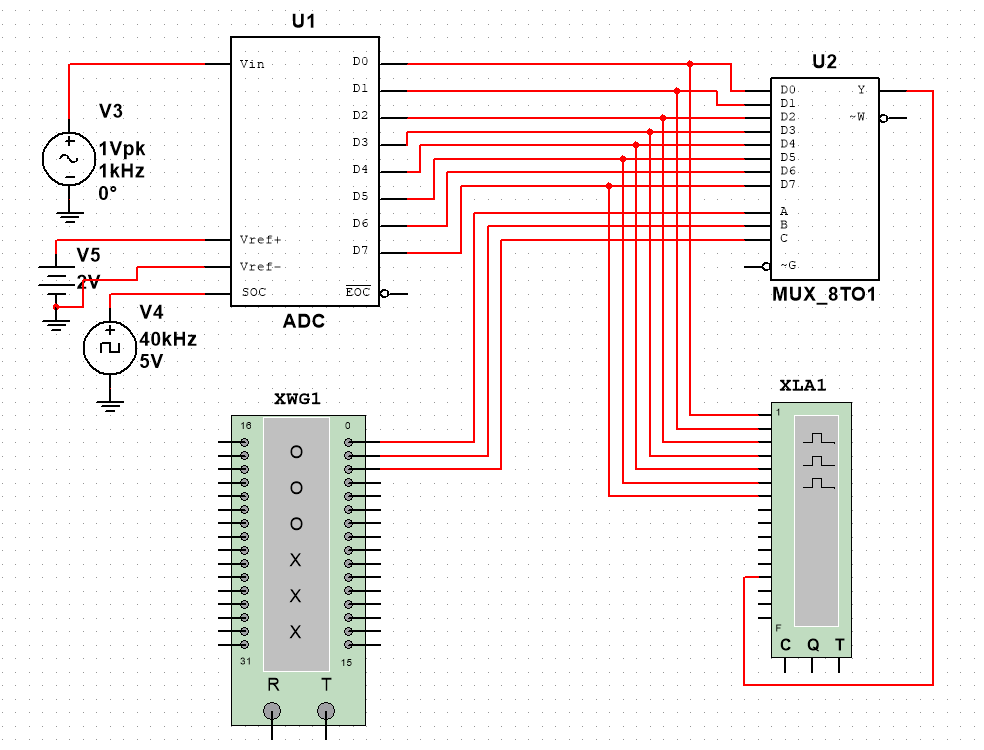
\includegraphics[width=0.75\textwidth]{images/digitalizacion_circuito.png}
    \caption{Circuito del sistema de codificación PCM con ADC de 8 bits, multiplexor 8 a 1, generador de palabras y
             analizador lógico.}
    \label{crkt.ej4:digitalizacion}
\end{figure}

El sistema está conformado por los siguientes bloques:
\begin{itemize}
    \item Fuente senoidal de entrada $V_3$: señal analógica de $1\,\unit{\volt_\mathrm{pk}}$ y frecuencia de $1\,\unit{\kilo\hertz}$.
    \item Conversor analógico-digital $U_1$ (ADC): convertidor de 8 bits alimentado con tensiones de referencia
          $V_{\mathrm{ref}+} = 2{,}0\,\unit{\volt}$ y $V_{\mathrm{ref}-} = 0{,}0\,\unit{\volt}$.
    \item Reloj de muestreo $V_4$: tren de pulsos de $5\,\unit{\volt}$ y frecuencia $f_s = 40\,\unit{\kilo\hertz}$
          conectado al terminal SOC (Start Of Conversion) para gobernar la cadencia de muestreo del ADC.
    \item Multiplexor digital $U_2$ (MUX\_8TO1): dispositivo selector de 8 canales a 1 salida, cuyas entradas de datos
          se conectan a las salidas paralelas del convertidor.
    \item Generador de palabras digitales (XWG1): provee una secuencia cíclica ascendente de 3 bits ($000_2$ a $111_2$)
          conectada a las líneas de dirección A, B y C del multiplexor para serializar la palabra binaria dentro de cada
          período de muestreo.
    \item Analizador lógico (XLA1): registra en forma sincrónica las líneas paralelas del ADC y la salida serializada.
\end{itemize}

A partir de los valores del circuito, los parámetros característicos de la digitalización resultan:
\begin{itemize}
    \item Fondo de escala: $V_{\mathrm{FSR}} = V_{\mathrm{ref}+} - V_{\mathrm{ref}-} = 2{,}0\,\unit{\volt}$.
    \item Cantidad de niveles discretos: $L = 2^8 = 256$ niveles.
    \item Paso de cuantización: $q = V_{\mathrm{FSR}} / 256 = 7{,}8125\,\unit{\milli\volt}$.
    \item Tasa de bits de la trama serie: $R_b = 8 \text{ bits} \cdot 40\,\unit{\kilo\hertz} = 320\,\unit{\kilo\bit\per\second}$.
    \item Duración de cada bit: $T_b = T_s / 8 = 25\,\unit{\micro\second} / 8 = 3{,}125\,\unit{\micro\second}$.
\end{itemize}

\section{Resumen Temporal en los Puntos G y H}
En la figura \ref{fig.ej4:adc_logic_analyzer} se muestra la captura obtenida en el analizador lógico virtual XLA1 para
los puntos de medición G y H fijados por la consigna.

\begin{figure}[!ht]
    \centering
    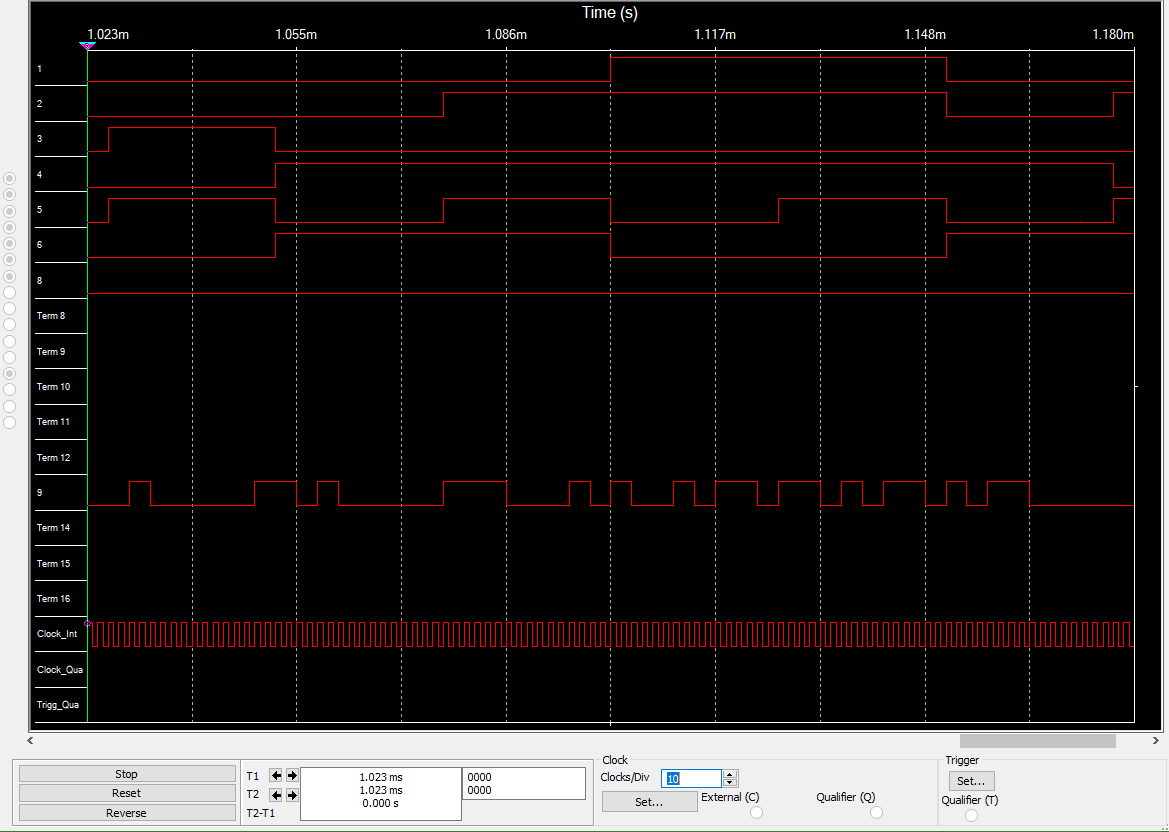
\includegraphics[width=0.75\textwidth]{images/adc_logic_analyzer.png}
    \caption{Resumen temporal en el analizador lógico: bus paralelo del ADC en el punto G (canales 1 a 8), trama digital
             serie en el punto H (canal 9) y reloj interno de sincronismo.}
    \label{fig.ej4:adc_logic_analyzer}
\end{figure}

El análisis de las señales registradas permite observar:
\begin{itemize}
    \item \textbf{Punto G (Canales 1 a 8, bus paralelo $D_0$ a $D_7$):} Representa la palabra binaria cuantizada a la
          salida del ADC. Las líneas $D_0$ a $D_2$ (bits de menor peso o LSBs) conmutan con alta frecuencia debido a su
          resolución de pocos milivolts ante las pendientes de la señal analógica. En contraposición, las líneas $D_5$ a
          $D_7$ (bits de mayor peso o MSBs) presentan transiciones estables y de menor cadencia, describiendo el ciclo
          fundamental de la onda senoidal de entrada de $1\,\unit{\kilo\hertz}$. Las actualizaciones del bus ocurren de
          forma sincrónica en cada flanco de muestreo del pulso SOC ($T_s = 25\,\unit{\micro\second}$).
    \item \textbf{Punto H (Canal 9, terminal Y):} Muestra la trama digital serie resultante a la salida del multiplexor
          $U_2$. El barrido de las entradas de selección A, B y C del multiplexor a través del generador de palabras
          recorre secuencialmente las líneas $D_0$ a $D_7$ durante el período de muestreo, conformando un flujo serie de
          pulsos lógicos binarios de duración constante $T_b = 3{,}125\,\unit{\micro\second}$.
    \item \textbf{Canal de reloj (`Clock\_Int`):} Registra la base de tiempos del analizador con un ajuste de 10 clocks
          por división, verificándose la estabilidad de los niveles lógicos y la sincronía entre la palabra paralela y
          la trama serie transmitida.
\end{itemize}
